
\section{Baseline BGP Performance}

Baseline measurements of BGP performance target the central scale factors of complex BGP deployments: route table size---measured in terms of numbers of paths, prefixes, and source peers. A BGP speaker's software tables scale directly with these parameters.

\subsection{Key Questions}

Valid enquiries are:
\begin{itemize}
    \item How long does it take for the target system to process the routes it receives?
    \item Once it has built the tables, do these scale factors affect its ability to perform routing operations?
\end{itemize}

Related questions address how the structure of routing updates affects processing capacity and performance. Specific questions to be explored include:
\begin{itemize}
    \item Does initial table transfer time scale linearly with the number of peers?
    \item Are bursts handled as quickly when multiple active peers are connected?
    \item Are continuous mode measurements consistent with burst mode?
    \item Do different BGP implementations have different performance envelopes depending on the measurement criterion (initial table, burst, rate)?
\end{itemize}

\section{Test Programmes}

\subsection{Initial Table Transfer}
For each target platform, measure the time taken to process a full route table:
\begin{itemize}
    \item as the route table varies in total size (measured by prefixes and paths).
    \item as the route table structure varies in terms of paths, holding table size constant.
    \item as the group size (number of prefixes per announcement) varies, holding the number of paths constant.
\end{itemize}

\subsection{Effect of Update Packing}
Repeat the initial table transfer measurements while disabling the packing of prefixes and compare the results.

\subsection{Stable State, Burst Processing Performance}
Measure the duration of processing bursts of updates of varying sizes. Repeat these measurements with variations in the route structure, using a subset of the values from the initial transfer tests.

\subsection{Rate-Based Measurements}
In each scenario where burst performance has been measured, substitute a continuous stream of updates.

\subsection{Effect of Multiple Peers}
Repeat a subset of all the above measurements in scenarios with multiple active source peers.

\subsection{Sensitivity to Experimental Parameters}
Explore sensitivity to experimental parameters, such as:
\begin{itemize}
    \item rate window size.
    \item burst repetition interval duration.
\end{itemize}

\section{Analysis and Hypotheses}

\subsection{General Expectations}
\begin{itemize}
    \item Larger inputs are expected to take more time to process, but the relationship should be no more than linear.
    \item With a larger installed routing state (table size, number of peers), burst and rate mode measurements might show a performance decline. However, this decline should be sub-linear if the software structure is moderately well designed.
    \item There may be multiplier effects between, for example, the number of peers and the size of the route table.
\end{itemize}

\subsection{Packing and Update Structure}
\begin{itemize}
    \item Route tables with fewer paths (larger group size) might yield better performance. However, there could be trends in both directions: large groups may require more work to construct announcements (poorer performance), while also reducing message-level overhead such as parsing (better performance).
    \item If packing is disabled, the performance for tables with a high group size is expected to decline to the performance of a table composed entirely of singletons (assuming such tables perform worse). This might lead to the conclusion that only the prefix count matters, apart from the gain accruing from reduced overhead in iterating over fewer Update messages.
    \item Distributing load (burst or continuous) over multiple peers is expected to improve performance if the target system has concurrent processing capabilities. If not, some mild disadvantage might be observed when working with loads over multiple peers.
\end{itemize}

\section{Test Framework: Kakapo, Kagu, and Forest}

For most of the proposed experiments, each `data point' represents a single invocation of the \texttt{kakapo} core binary application and an instance of the target BGP speaker. The \texttt{kagu} framework provides the orchestration of the various BGP instances (usually, as \texttt{Docker} containers).

Part of \texttt{kagu}/\texttt{kakapo} is an experiment configuration template system named \texttt{forest}. The complete workflow is as follows:
\begin{enumerate}
    \item \texttt{forest} takes a \texttt{YAML} file that defines the range of parameters needed, along with any invariants. The output of \texttt{forest} is a series of shell commands that drive the \texttt{kagu} runtime framework. Each command line differs from the others only in the parameters set to vary, for example, the \texttt{table-size} and the target BGP speaker.

    \item \texttt{kagu} is invoked once for each line in the script file. It builds the needed network interfaces and address mappings for the BGP systems it will start. It then constructs the \texttt{Docker} commands (or \texttt{libvirt/virsh}) to start the BGP endpoints---one is always a \texttt{kakapo} container, the other varies depending on the BGP target named in the command line. \texttt{kagu} transcribes the parameters directed at \texttt{kakapo} (for example, the table size) into the command parameters that \texttt{kakapo} needs, which are then passed explicitly into the \texttt{Docker} container. By careful crafting, the BGP platform-specific configuration files need not be changed for any of the experiments.

    \item \texttt{kakapo} is run as a container in the foreground rather than as a daemon, which allows it to control the experimental lifecycle. It executes the configured test and exits when complete, or on error. \texttt{kakapo} is started with a logging file mapped into the container; this file records the progress and results of the instance. \texttt{kakapo} sets signal handlers that allow it to exit gracefully, even if an exception arises in its own code.
\end{enumerate}

This process allows for the management of very long-running experiments, even in the event of system outages. \texttt{forest} scripts can be restarted because they contain sequence numbers that are recorded in the logging file. As long as the host file system is not corrupted, no experimental data can be lost.


% Baseline measurements of BGP performance target the central scale factors of complex BGP deployments:
% route table size - measured in terms of numbers of paths, numbers of prefixes and numbers or (source) peers.
% A BGP speaker of necessity has software tables that correspond to directly in scale to these parameters.

% Valid enquiries are:
% \begin{itemize}
%     \item how long does it take for the target system to process the routes it receives
%     \item once it has built the tables, do these scale factors affect its ability to perform routing operations?
% \end{itemize}

% Related questions address how the structure of routing requests affect the processing capacity and performance in completing those requests.

% Concrete test programs:

% Initial table transfer

% for each target platform, measure the time taken to process a full route table
% \begin{itemize}
%     \item as the route table varies in total size (measured by routes~prefixes)
%     \item  as the route table structure varies in terms of paths
%     \item \begin{itemize}
%      \item  holding table size constant
%     \item  holding group size constant
%     \end{itemize}
% \end{itemize}

% Effect of Update packing

% Repeat and compare the same measurements, whilst disabling packing of prefixes.

% Stable state, burst processing performance

% measure the duration of processing bursts of updates of varying sizes.
% repeat the measurements with variations in the route structure (using some subset of the values in part 1)

% Effect of multiple peers
% Repeat some subset of all of the above measurements, in scenarios with multiple active source peers.
% Does initial table transfer time scale linearly?

% Are bursts handled as fast, when multiple active peers are connected?

% Rate based measurements

% In each scenario in which burst performance has been measured, substitute continuous mode.
% Are the continuous mode measurements consistent with burst mode?
% Do the different BGP implementations have different performance envelopes depending on the measurement criterion (initial table, burst, rate.)

% Sensitivity to experimental parameters
% explore
% - sensitivity to rate window size
% - to burst repetition interval duration

% Analysis, Hypotheses
% We should expect that larger inputs generally take more time to process, but no more than with linear relation.
% We might expect that having a larger installed routing state (size of table, number of source peers), that burst and rate mode measurement show some variation (performance decline).  But sublinear, if the software structure is even moderately well designed.
% We might expect that their are multiplier effects between, for example numbers of peers and size of route table.

% Packing and update structure
% We might expect that route tables with fewer paths (larger group size) have better performance, but there could be trends in both directions, e.g. large groups may require more work to construct announcements, leading to poorer performance, while the same variation might contribute to better performance in the area of processing where there is a message level overhead, for example in parsing an update, and in reducing the size of a `path table', if such a thing exists in the target implementation.
% We might expect that if packing is disabled that the performance for high group size tables declines to the performance of an all singleton table (assuming that such tables do have worse performance.)
% This might lead to the conclusion that only prefix count matters, excepting the `trivial' gain accruing from reduced overhead in iterating over more Updates.
% We might also expect that distributing load (burst or continuous), over multiple peers, would lead to better performance, if, and only if, the target system has some concurrent processing capability - but if, not then perhaps some mild degree of disadvantage when working with loads over multiple peers.

% Configuring and Analysing Results In A Kakapo Test Campaign
% For most of the proposed experiments, each `data point' represents a single invocation of the kakapo core binary application, and also of an instance of the target BGP speaker.  The kagu framework provides the orchestration of the various BGP instances (usually, as Docker containers).

% kagu, kakapo and forest

% Part of kagu/kakapo is an experiment configuration template system which builds a sequence of test scripts which in aggregate represent the tests needed.  The tool is `forest' - the complete picture is as follows:
% forest takes a yaml file which defines the range of parameters needed, and also any invariants -the output of forest is a series of command lines (Linux shell commands) which drive the kagu runtime framework.  Each line differs only from the others in the batch in the parameters which are set to vary - for example, the table-size, and the target bgp speaker.
% kagu is invoked once for each line in this script file - kagu builds the needed network interfaces and address mappings for the BGP systems that it will start, and then constructs the Docker commands (or libvirt/virsh) which will start the BGP endpoints - one of them always a kakapo container, the other varies, depending on the BGP target named in the command line.  kagu transcribes the parameters which are directed at kakapo (for example, the table size) - into the command parameters that kakapo needs.  These are passed into the Docker container explicitly by kagu.  In this way, kakapo is configured and started, as a container, along with the target BGP speaker (BGP speakers each have there own configuration files, but by careful crafting, these BGP platform specific files need not be changed for any of the experiments known to kagu and forest).
% Although Kakapo is run as container, it is run in the foreground rather than as a daemon, this allows kakapo to control the experimental lifecycle.  Kakapo executes the configured test, and exits when complete, or on error or exception, terminating the container.  Kakapo is started with a logging file mapper into the container, and this updated file records the progress and results of the experimental instance, including when kakapo exits (kakapo sets signal handlers which allow it to gracefully exit, even if the exception arises in its own code.)

% Forest scripts can even be restarted, because they contain sequence numbers, and the sequence numbers are recorded in the logging file.  The procedure is manual, but trivial, and allows very long running experiments to be managed, even in the event of system outages.  And, of course, as long as the hist file system is not corrupted, no experimental data can be lost.

\section{Reported Experimental Program}

In the interest of space and relevance, only a limited selection of experimental reports is given.

\paragraph{The first report} corresponds to the initial findings during the development of both kakapo and \hbgp.
It is the measurement of initial transfer duration for some `representative' sized routing tables, followed by the simple measurement of burst performance, in the context of this specific `representative'  route table.

In the initial work, the range of BGP speakers was limited (no Cisco or Junos virtual routers), and older versions of almost every BGP platform than reported here.  It's noteworthy that gobgp in particular is now demonstrably more mature, in that it is now possible to conduct most measurements, whereas in earlier times gobgp could not be reliably tested with full route tables and loads such as these.

Here are the `forest' YAML files which define these initial experiments \footnote{`forest' did not exist when these experiments were first conducted, however another orchestration system was in use - Haskell based (`forest' is Python!  The Haskell framework was not so easy to use and modify.) }

This is the content of the `forest' YAML file for the first experiment: \inputminted{yaml}{specs/burst1.yaml}


At the risk of stating the obvious, the specification requests that a set of experiments be conducted using the bgp speakers bird1, bird2, bird3, frr, hbgp, bgpd, gobgp, relay, with a route table size of 800000 (prefixes).
The meaning of the remaining lines is as follows:

\verb|  MAXBURSTCOUNT: "10000"|
\verb|MODE: SINGLE| - kakapo experiment mode is defined here
\verb*|  REPEAT: "5"| instructs that the burst test should be executed 5 times,
\verb|spec: forest| is a signature line - the `forest' script will reject the input of it is missing.

There are two comment lines - 
\begin{verbatim}
  # GROUPSIZE: 1..10
  # NOPACK: 0,1    
\end{verbatim}

which are placeholders for hopefully obvious variations on the file for a future similar experiment, and the remaining non-comment lines are tags of sorts which do not affect the experiment, but help to track and distinguish the recorded data for later analysis.

The script forest transforms this YAML file into the following lines of Linux shell script:
% \begin{adjustbox}{max width=\textwidth}
% { \fontsize{6pt}{9.6pt}\selectfont
% \begin{lstlisting}
\begin{lstlisting}[basicstyle=\fontsize{10pt}{16pt}\selectfont\ttfamily]


    

SEQ=0 SPEC=burst1 TAG=EXAMPLE_burst1 REPEAT=5 MAXBURSTCOUNT=10000 PREFIXCOUNT=800000 MODE=SINGLE target=bird1 /home/nic/kakapo/testing/smoketest/runx.sh
SEQ=1 SPEC=burst1 TAG=EXAMPLE_burst1 REPEAT=5 MAXBURSTCOUNT=10000 PREFIXCOUNT=800000 MODE=SINGLE target=bird2 /home/nic/kakapo/testing/smoketest/runx.sh
SEQ=2 SPEC=burst1 TAG=EXAMPLE_burst1 REPEAT=5 MAXBURSTCOUNT=10000 PREFIXCOUNT=800000 MODE=SINGLE target=bird3 /home/nic/kakapo/testing/smoketest/runx.sh
SEQ=3 SPEC=burst1 TAG=EXAMPLE_burst1 REPEAT=5 MAXBURSTCOUNT=10000 PREFIXCOUNT=800000 MODE=SINGLE target=frr /home/nic/kakapo/testing/smoketest/runx.sh
SEQ=4 SPEC=burst1 TAG=EXAMPLE_burst1 REPEAT=5 MAXBURSTCOUNT=10000 PREFIXCOUNT=800000 MODE=SINGLE target=hbgp /home/nic/kakapo/testing/smoketest/runx.sh
SEQ=5 SPEC=burst1 TAG=EXAMPLE_burst1 REPEAT=5 MAXBURSTCOUNT=10000 PREFIXCOUNT=800000 MODE=SINGLE target=bgpd /home/nic/kakapo/testing/smoketest/runx.sh
SEQ=6 SPEC=burst1 TAG=EXAMPLE_burst1 REPEAT=5 MAXBURSTCOUNT=10000 PREFIXCOUNT=800000 MODE=SINGLE target=gobgp /home/nic/kakapo/testing/smoketest/runx.sh
SEQ=7 SPEC=burst1 TAG=EXAMPLE_burst1 REPEAT=5 MAXBURSTCOUNT=10000 PREFIXCOUNT=800000 MODE=SINGLE target=relay /home/nic/kakapo/testing/smoketest/runx.sh

\end{lstlisting}

% \end{adjustbox}

 Fortunately for the reader, there is only one range parameter in this input, and the range is small, resulting in just eight script lines.
 But, when the comment lines\begin{verbatim}
  # GROUPSIZE: 1..10
  # NOPACK: 0,1    
\end{verbatim}

are converted to active configuration - 

\begin{verbatim}
  GROUPSIZE: 1..10
  NOPACK: 0,1    
\end{verbatim}

Then the resulting script will have 160 lines, and may take rather longer to execute than this version.

We now show the output in the console, and later some fragments of the structured log file, arising from executing these scripts.

(Incidentally, this complete set of experiments executes in around 5 minutes.
The fastest BGP speaker runs in 31 seconds, the slowest, gobgp, takes a little more than one minute.  bird2, the next fastest, takes 32 seconds, although it is still 10x slower than the fastest, our reference BGP, `relay'.  Even though gobgp now completes most tasks, it is still much the slowest of all of the `software' BGPs (Cisco and Juniper VMs will be discussed later.))

With only a few lines redacted, here is the complete console log of one of the execution cycles, in this particular case the BGP target was FRR.

\begin{figure}[H]
\begin{adjustbox}{}

\begin{lstlisting}[numbers=left]
kakapo  version: 1.0-743-g876b50d  built: Tue Jun  3 05:55:51 UTC 2025  branch: main
connecting from 172.18.0.19 to 172.18.0.13:45824 (179) (0)
connecting from 172.18.0.20 to 172.18.0.13:45824 (179) (0)
connection initiated for 2 peers

BGP Open: as = 64504, routerid = 172.18.0.13 , holdtime = 180, opt params = 0206010400010001020280000202020002024600020641040000fbf8020206000206450400010101020a490806616c656630310002044002c0780209470700010180000000
BGP Open: as = 64504, routerid = 172.18.0.13 , holdtime = 180, opt params = 0206010400010001020280000202020002024600020641040000fbf8020206000206450400010101020a490806616c656630310002044002c0780209470700010180000000
connection complete for 2 peers
conditioning start
conditioning:          peer 1 64504:172.18.0.20
conditioning complete: peer 1 64504:172.18.0.20  elapsed time 4.360066
conditioning complete: elapsed time 4.403960
canary for peer 1 64504:172.18.0.20
canary_all complete: elapsed time 0.050753
cycle 0
single_peer_burst_test total elapsed time 0.513073 count 100000 (transmit 0.005274) (receive 0.512899)
canary for peer 1 64504:172.18.0.20
canary_all complete: elapsed time 0.050711
cycle 1
.........

..........
cycle 4
single_peer_burst_test total elapsed time 0.508013 count 100000 (transmit 0.010109) (receive 0.507823)
canary for peer 1 64504:172.18.0.20
canary_all complete: elapsed time 0.050845
single_peer_burst_test mean=0.494902 max=0.522436 min=0.474067
Notification complete: elapsed time 0.000143
notification complete for 2 peers
kakapo exit
killed frr
\end{lstlisting}
\end{adjustbox}
\end{figure}
% BGP Open: as = 64504, routerid = 172.18.0.13 , holdtime = 180, opt params = 0206010400010001020280000202020002024600020641040000fbf8020206000206450400010101020a490806616c656630310002044002c0780209470700010180000000
% BGP Open: as = 64504, routerid = 172.18.0.13 , holdtime = 180, opt params = 0206010400010001020280000202020002024600020641040000fbf8020206000206450400010101020a490806616c656630310002044002c0780209470700010180000000

Some commentary: 
AT line 1 we see the kakapo start log output, with its version information (this will also be found in the structured log file)
At lines 6-8 the BGP peer associations that have been formed.  kakapo doesn't understand what the BGP Open options mean, but it can be given a special instance to send, if required.
At lines 9-12 we see the conditioning phase, i.e. the initial table transfer .
An additional interesting measurement here is the transmit time for each BGP peer, which is present in the log, for each BGP peer in turn, but the console is only reporting an aggregate, and we see here the total duration, from start of sending to end of receiving the re-announcement of the initial table for all peers.
At lines 13-14 the canary route exchange is reported - arguably canary here is redundant, but it is used widely to give confidence that each experimental stage has been completed.  Canaries are single routes.  Note that, for FRR, the smallest transaction always takes around 50 mS, because of all BGPs, FRR is the only one which does not disable Nagle.
At lines 19, the real `test' starts, and the number of cycles are as requested in the forest configuration. 
The report shows two numbers - (transmit 0.005274) (receive 0.512899) -  which added compose the aggregate - 0.513073.  As noted, FRR never takes less than 50mS for any transaction, so, for FRR, with this request size - 10,000 routes - the experiment is in some sense void.
The more relevant datum is the initial transfer time - 4.3 seconds - which is one of the slowest in the pack.   

We now show the structured log entry which was generated from this test cycle:

\begin{lstlisting}[    numbers=left]

    {
        "type": "summary",
        "unixtime": 1749509284,
        "elapsed_time": 36.951536,
        "test_name": "single_peer_burst_test",
        "time": "2025-06-09 22:48:04.412000",
        "sender_count": 1,
        "conditioning_duration": 4.17579,
        "mean": 0.486382,
        "max": 0.517761,
        "min": 0.474661,
        "sd": 0.01814,
        "PATHCOUNT": 80000,
        "PREFIXCOUNT": 800000,
        "GROUPSIZE": 10,
        "MAXBURSTCOUNT": 10000,
        "REPEAT": 5,
        "NOPACK": 0,
        "RATECOUNT": -1,
        "RATETIMELIMIT": 20,
        "single_rate": 0,
        "multi_rate": 0,
        "BRANCH": "main",
        "VERSION": "1.0-743-g876b50d",
        "HOSTNAME": "tauben",
        "UUID": "03ba4f38-445d-4eed-a8fe-57c7f79f697f",
        "exit_status": "NOT SET",
        "target": "frr",
        "TAG": "EXAMPLE_burst1",
        "SEQ": "8",
        "SPEC": "burst1",
        "N_PEERS": "1",
        "PSU_STATUS": "AC",
        "DOCKER_NCPUS": "16",
        "DOCKER_MEMORY": "96g",
        "WINDOW": 5000
    },
\end{lstlisting}

This record holds all of the relevant context of a test run, as well as the test control parameters and measured values.
The additional data is the environment and results.
For example, we can see that this run was in a Docker environment with 96G bytes of system memory and 16 CPUs.
Kakapo is not smart enough to choose which results to report depending on what test mode, so the meaning full data here is in the fields

\verb|"conditioning_duration": 4.17579|

\verb|"mean": 0.486382|

\verb|"max": 0.517761|

\verb| "min": 0.474661|

\verb| "sd": 0.01814|

 while
 
 \verb| "single_rate": 0|
 
 \verb| "multi_rate": 0,|
 
 are zero because the test was not a rate test.

 Every test run has a unique UUID, so that other records can be correlated with the final `summary' record, e.g., records such as start, and intermediate records that contain the measurements for each run, rather than just the means logged here.  Most other fields are self explanatory, e.g. `host' and `time'.


\section{Experimental Data Reporting and Presentation}

Previously, the methodology for definition and collection of experimental data was described, which consists of structured data sets in which most of the collected data values are `met-data' context for core experimental measurement values.

In order to effectively report and analyse this data, some form of automation is required.
The approach developed is described here.

\paragraph{Reporting Requirements}
The usual objective in reporting is to produce some form of graphical display, or a summary table, highlighting the relevant control variables and resulting experimental observations.
Since data is collected into a general pool, part of the requirement is to isolate and extract data records which are relevant to the topic; equally important for experimental integrity is to ensure that only directly comparable data is used in a single report, for example, that only data collected on a certain server, or in a certain experimental context, is used in a single report.


A side-effect of the selection phase is a summary of the metadata which is held fixed for the selected data, for example, the host name of the system used for the experiment, and any control parameters which are single valued for this report.  The metadata could also include the date ranges over which the data was collected, and software versions of any components in the experiment.


Once a valid subset of data values is isolated, the next objective is to construct the sets of index values - usually control parameters - and to form a regular representation of the measurements values, e.g., an n-dimensional matrix of measurements, in which index values are the `unit vectors' for the value matrix.

An intermediate step to forming this value matrix is the reduction of measurements from selected records to single data values: this may have two aspects:
\begin{enumerate}
    \item select which single value of several semantically distinct measurements present in the record
    \item summarise, e.g. calculate a mean (average), or some other format, such as an error-box structure
\end{enumerate}

Note, if more than one type of measurement is present in the data records, then this may also be interpreted as a dimension in the value matrix, for example when rate data is collected, each measured rate record also contains the measured duration for the `conditioning phase' of the experimental cycle. This could be used simply to create distinct graphs/reports, but if the complementary data should be plotted in the same report, then it should be processed as a dimension in this way.


Once this data reduction stage is complete a regular data structure is in hand, and the choices of graph ranges and axes labels etc are implicitly already determined, so that a graph or table is almost completely defined - the remaining task is to specify the graph or table type to apply, for example, line graphs or bar charts, etc.  The choices available may be restricted by the axes types, in particular, line graphs are only applicable to axes which are numeric, otherwise a bar chart may be a more meaningful format.
Therefore, in many cases the choice of graph form may already be implicit in the data selected.

\subsection{Reporting Implementation}
The foregoing analysis presents the requirements for a concrete framework for processing experimental data.  In this document the tool presented is a set of python scripts.  Earlier work utilised Haskell based approach, but the required graphical back end was based on libraries which have since fallen put of active development, so when the transition to JSON and MongoDB for data processing was developed a switch to python and `matplotlib' was also undertaken.  The report and graph generating framework is now part of the `kakapo' ecosystem, under the heading kakapo/report.

kakapo/report (`reports', hereafter), follows the structure set out already, i.e.

\begin{itemize}
    \item data ingestion (file or mongodb)
    \item data-set analysis and pre-processing
    \item
    \begin{itemize}
     produces a list of raw experimental data objects
    \end{itemize}
    \item dataset selection (and metadata summary preparation)
     \begin{itemize}
     \item produces a matrix structure with aligned axes vectors, the values are still raw experimental data objects
    \end{itemize}
    \item 'projection' phase
    \begin{itemize}
     \item reduce the structure raw data values to graphable values
     \item NB the projection may produce another data matrix dimension
    \end{itemize}
    \item rendering
    \item \begin{itemize}
     produce graphs or tables, using formats inferred or specified.
\end{itemize}
\end{itemize}

\subsubsection{Implementation Details}
\paragraph{Filters and Selectors}
Filters are rules (predicates) which partition the dataset, only the included elements (predicate=true) are considered for later processing.
Selectors define values used as axes values - they are rules which applied to values produce scalar values, either labels (strings), or numeric values.

In most cases, selectors and filters are simple functions which match or extract on keys in the raw data items.
Such filters most often takes key and a list of values, or a single value, while simple selectors most often take just a key.
But a selector might take a list of values as an inclusive or exclusive condition.
The fundamental difference between a filter is the output is boolean, which the selector is a value of type determined by key.
What they have in common is a key and, possibly empty, lists of inclusive or exclusive elements.
Even a filter could have empty lists, in which case the filter is on the presence (or absence) of the key itself.
The presence (or absence) of the key itself is always an implicit part of the function, and an absent key is a special value.
, for a filter it should be defined, but if there is an inclusive list in the filter then the key must be present, unless a null value is in an inclusion list.

Selectors and filters which do not fit this framework of working with keys and unprocessed values other than as equality candidates can be considered: but they are always of the form of predicate in the case of filters, or a function with a regular return type.  At this level, there is no real distinction between Filters and Selectors except that a filter should only return boolean values.  The class of such filters and selectors can be further subdivided - the simpler category being functions over a single key, while more general cases might depend on many keys in the raw data object.

\paragraph{Projectors}
At this point, the topic of projectors becomes relevant: a projector has been defined as an extractor of `y' values - and it is clear that Projectors share properties of Filters and Selectors.  The more significant distinctions being that they yield values which may be more complex than Filters and Selectors, and that, for some cases, the projector is required to implement an aggregation function.

Specifically, a Projector may have two sub-functions - 
\begin{enumerate}
    \item extract a numeric(?) value from a raw data object
    \item combine multiple extracted values to form a single `plottable' `y-value'
\end{enumerate}

 In reality, these functions can be treated independently, and the term Projector limited to the function which extracts values from raw data objects.  In this case, the Projector is much like Filters and Selectors in that simple cases can be just a key label which yields the corresponding value, and more complex cases follow the same lines as for Filters and Selectors, i.e. functions over single values, and functions over multiple values.

\paragraph{Aggregators}
 This leaves the final category of report function, which is the Aggregator.  An Aggregator may commonly be a function such as mean, sum, max or min, or even count; first, last, latest might be possible, but only if the Projector produces a structured value which for example, has a date field.  What it has always is a mapping from a type [T] to a type T.

\paragraph{ Combining Filters, Selectors, Projectors and Aggregators}

 Filters are candidates for combination, however the mechanism is ambiguous when more than one Filter is named: should AND or OR be used to combine them?  It is easy (in python, and other languages) to create a filter as a lambda of two filters, the problem comes when the member filters contain lists, and the requirement is to give the list as a command line parameter, or otherwise independent of the source code of the script.  The simplistic solution adopted is that when filters are aggregated, the implied meaning is that only elements matching every filter are passed.

 Selectors are simpler than Filters - A Selector always has a role, it may be just one of `X selector', `group selector' or `subgroup selector'.  There may at most one of each.  `group selectors' or `subgroup selectors' are optional.

 Similarly with Projectors and Aggregators, there be exactly one of each.  When a Projector produces two values, then the Aggregator is assumed to be applicable to both. [Could be made more flexible.]

 
\subparagraph{Projectors that produce multiple values}
 Projectors that produce multiple values create an implicit group or sub-group in the dataset.  The Projector defines the labels used for the subgroup itself.

\subsubsection{ Using the framework for real data and analysis}
 Until now, Filters, Selectors, Projectors and Aggregators are described in abstract terms - in practice, how should they be constructed and used?
 In practice a single combination of Selectors, Projectors and Aggregators may be applicable to a wide range of data, and thus many combinations of Filters.  Therefore, although Filters are logically relate to Selectors, Projectors and Aggregators, there usage diverges: and the divergence is reflected in the user interface; combinations of Selectors, Projectors and Aggregators are lumped into a class and concept called `view' (View objects).  View objects are widely reused, and also serve as a vehicle for carrying other data needed to construct graphs.  For a given type of View object there may be only a single applicable rendering into a graph, and certainly there can be some default prescribed as part of the View.

 Using Filters
 Evidently, a View may be a source-code level entity, while a Filter might be 'source-code' too, but one constructed dynamically rather than as a source-code literal.  For may cases, a sufficient filter specification can be defined as just a single predicate against a metadata field such as TAG or SPEC, possibly further restricted by naming a single host from which the data should be drawn.  Therefore, an invocation of a report generator may have the form:

\verb| $ report <data source> view=view1 filter=TAG=BURST1|

 or 
 
\begin{lstlisting}
$ report <data source> view=rate1 filter=TAG=RATE1,RATE2 filter=host=server1 filter=target=bird2,frr,hbgp
\end{lstlisting}
 where rate1 has been defined as:
\begin{lstlisting}

 {
  Selectors: {
    X: sender_count
    group: target
    subgroup: WINDOW
  }
  Projector: multi_rate
  Aggregator: mean
  Graph: G_line_1
 }
\end{lstlisting}

\subsection{ Report Management}
 The report tool produces graphs or tables on demand, based on command line filters and other directives.
 It is useful to easily save a report for posterity, with metadata, so that it may be repeated and validated, or reapplied when additional experimental data is available.
 The report tool facilitates this by creating archives on request, the archive contains the command used to create the plot, the figure generated, the associated metadata, and the selected raw data which formed the basis of the report.

 The effect is that any quoted result can be traced back to the original data, and the plot regenerated exactly, or run again with later data using the save command.

 An example will serve to illustrate the usage - here the data produced using the previously described experiment specification in the `forest' tool is displayed in graphical form.
 The forest specification file contained a `TAG' value, which we can use to extract just the data produced for that request.  The command line to do this is:

\begin{lstlisting}
$ ./report2.py mongo tag=EXAMPLE_burst1 opt=bar save
\end{lstlisting}
 and the resulting output (slightly truncated)I is this:

\begin{lstlisting}
Debug filter
filter recent reject_count=851 accept_count=100441 except_count=0
filter exclude_targets reject_count=93 accept_count=101199 except_count=0
filter filter_on_tags reject_count=101224 accept_count=68 except_count=0
End - Debug filter
*** rejected 101224/101292!!!

===================
Post Filter Summary
===================
summarising 68 items
sample data time window is 2025-06-10 - 2025-06-11
key: test_name [single_peer_burst_test(67)]
key: PREFIXCOUNT [800000(67)]
key: GROUPSIZE [10(67)]
key: BRANCH [pathcount(39), experimental(24), forest(2)]
key: VERSION [1.0-746-gd06d05d(48), 1.0-747-g6edd416(7), 1.0-748-gdf37aea(3), 1.0-749-ga63b427(3), 1.0-743-g876b50d(2)]
key: HOSTNAME [alef01(67)]
key: target [frr(10), bird1(8), bird2(8), bird3(8), hbgp(7), bgpd(7), relay(6), gobgp(6)]
key: TAG [EXAMPLE_burst1(67)]
key: SPEC [burst1(67)]
key: BURSTSIZE [10000(67)]
===================
***no missing cells!!!
*** duplicate cells in {'7 repeated x in relay:10', '8 repeated x in bgpd:10', '8 repeated x in hbgp:10', '9 repeated x in bird1:10', '9 repeated x in bird3:10', '7 repeated x in gobgp:10', '9 repeated x in bird2:10', '11 repeated x in frr:10'}
*** 8 elements in plot (raw=68) (@project_y)
 graph was saved to /tmp/tmptbem1tzv.png
command line was "./report2.py mongo tag=EXAMPLE_burst1 opt=bar save"
command line was ./report2.py mongo tag=EXAMPLE_burst1 opt=bar save
save dir is  /home/nic/.kakapo/1750178719

\end{lstlisting}    

 Notice from the first few lines that the database itself contains 101292 records, of which only a very few match the tag given - `EXAMPLE_burst1'.

 The generated graph \ref{fig:1750178719} for this simple experiment and analysis is shown here.

 \begin{figure}[H]
    \centering
    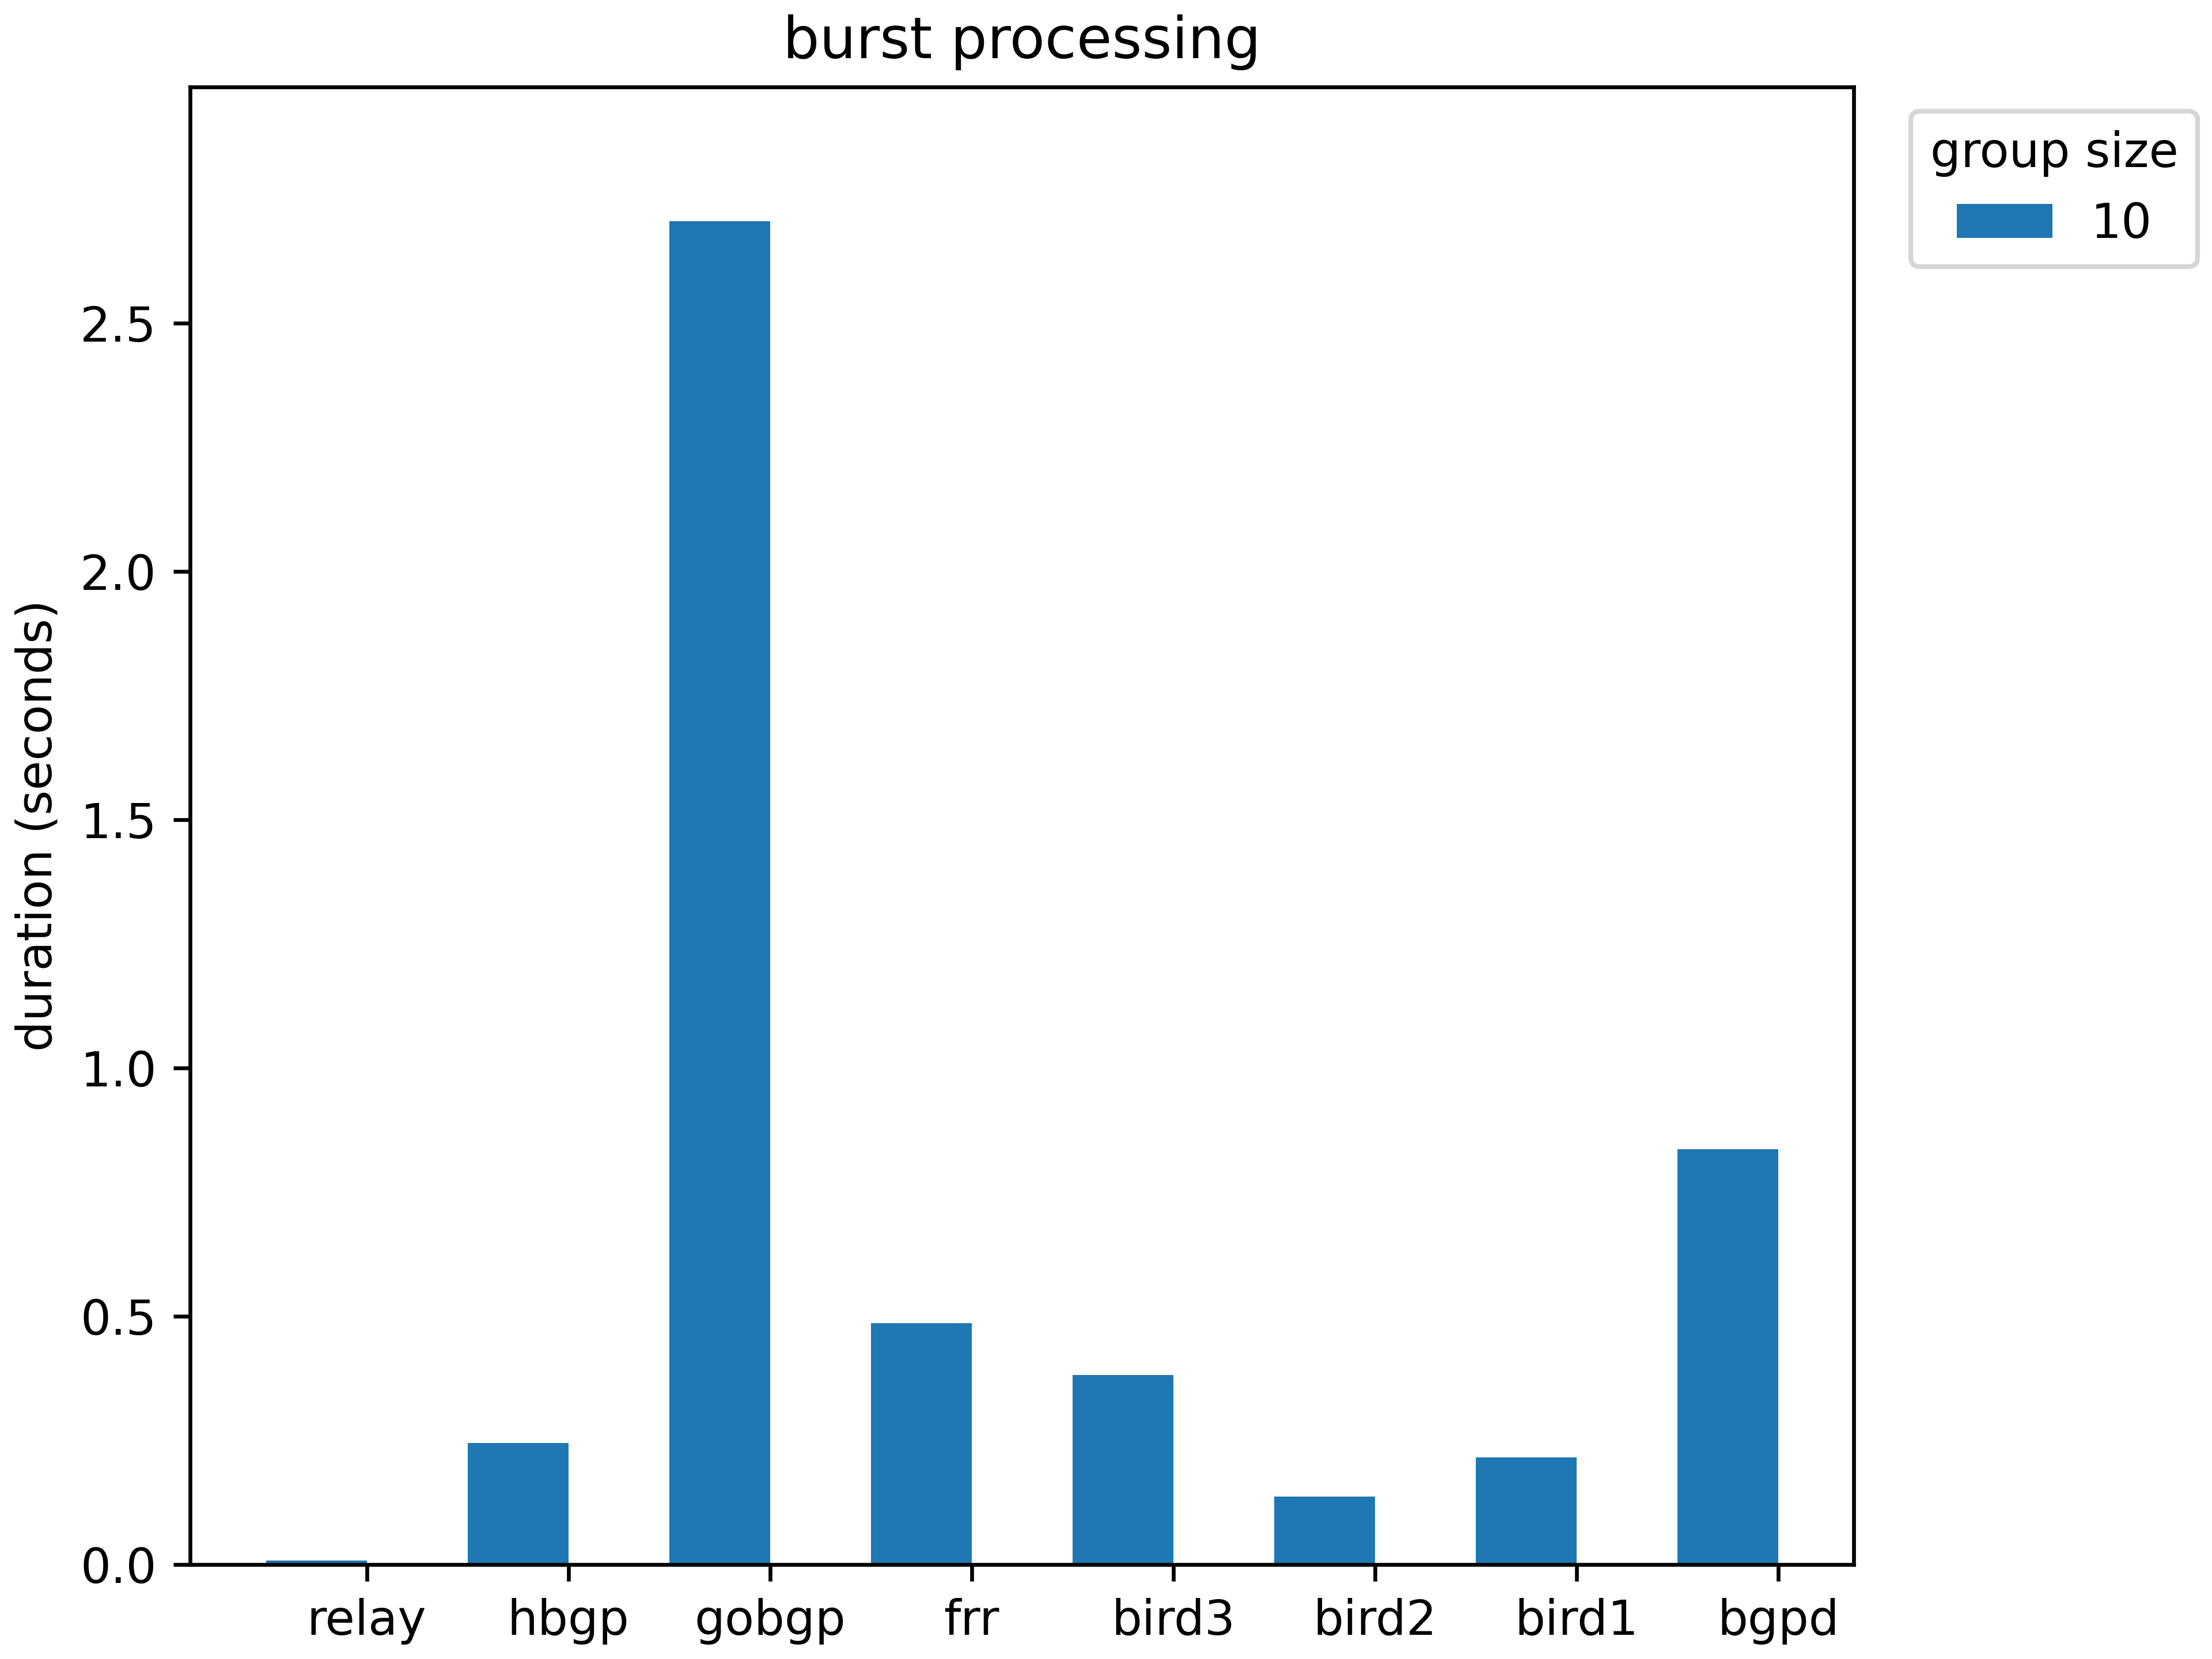
\includegraphics[width=0.7\linewidth]{1750178719.png}
    \caption{sample figure from report tool}
    \label{fig:1750178719}
\end{figure}

A more complete example is this one: \ref{fig:1750175110}.
for which the command was:
    \begin{lstlisting}
    ./report2.py mongo host=alef01 tag=samples3 targets=bird1,bird2,bird3,frr,hbgp,bgpd,gobgp save
    \end{lstlisting}

  \begin{figure}[H]
    \centering
    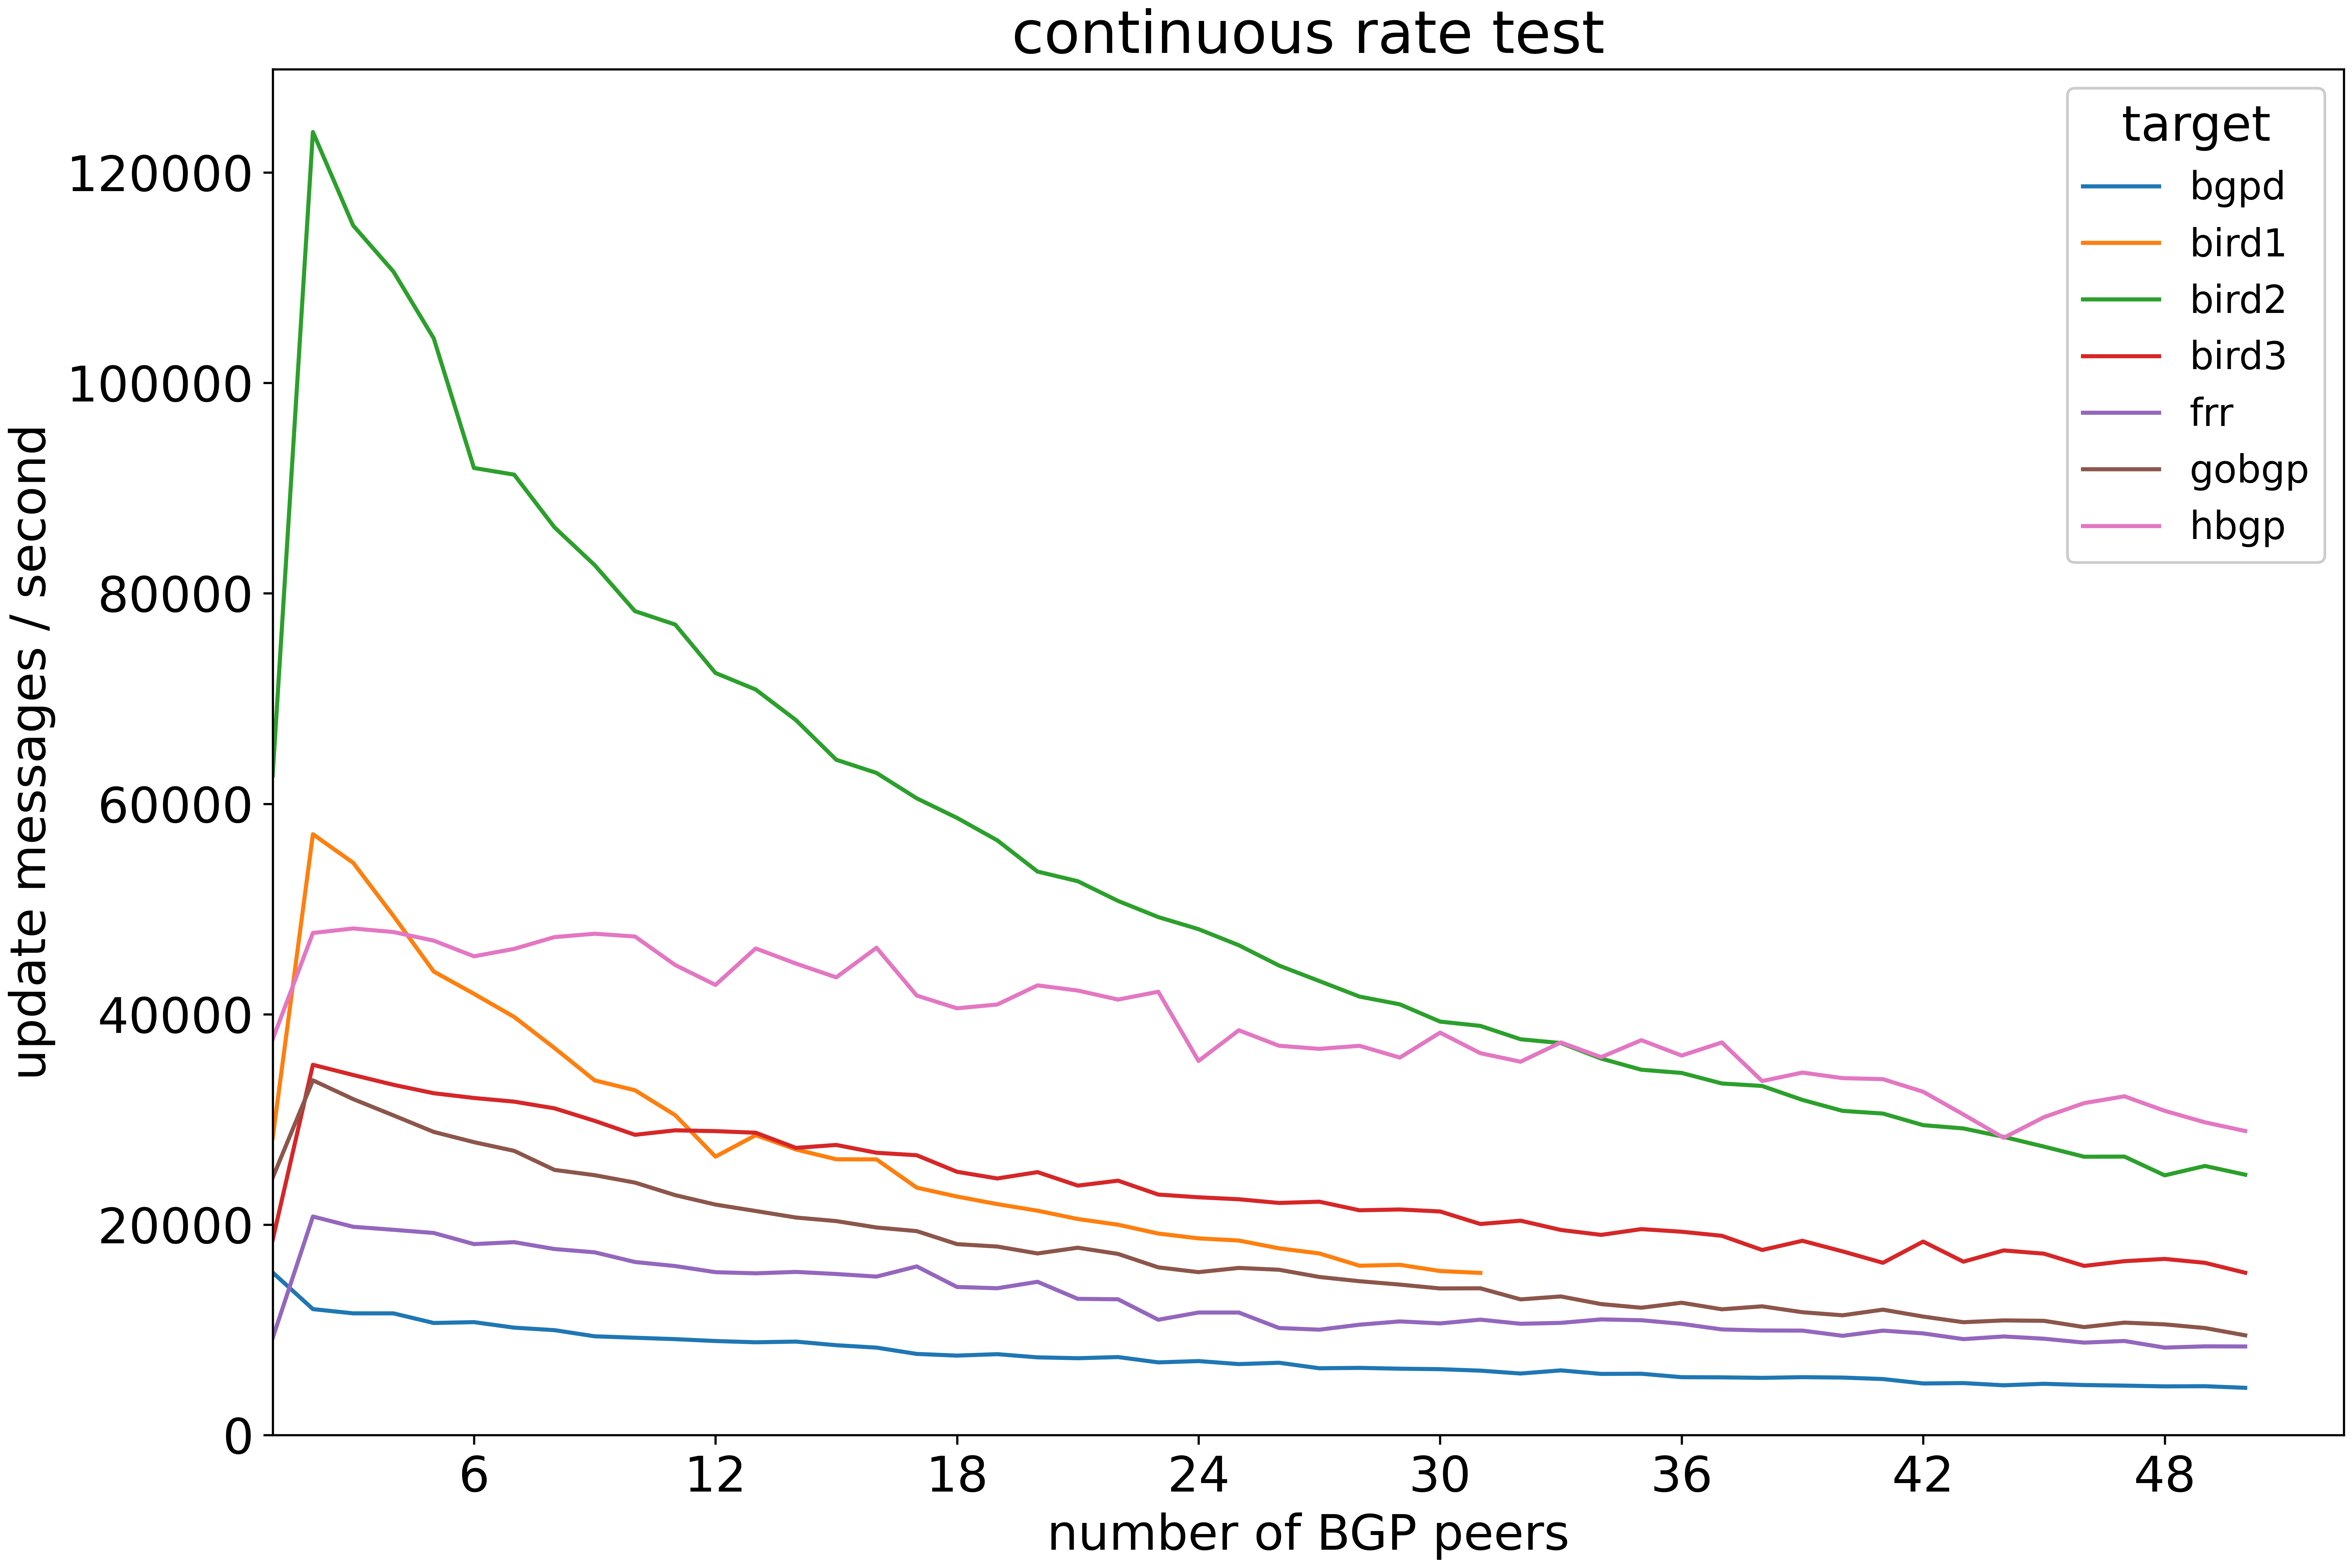
\includegraphics[width=0.7\linewidth]{1750175110.png}
    \caption{sample figure from report tool    }
    \label{fig:1750175110}
\end{figure}


